\newcommand*{\PathToAssets}{../assets}%
\newcommand*{\PathToOutput}{../output}%
\documentclass{article}
\usepackage[a4paper, margin=1in]{geometry}
\usepackage{graphicx}
\usepackage{caption}
\usepackage{float}

\title{Data Retrieval and Analysis Report}
\author{Aadi Deshpande}
\date{\today}

\begin{document}

\maketitle

\section{Introduction}
This report summarizes the process of retrieving, preprocessing, and analyzing financial data from multiple sources. The datasets include call reports, treasuries, and MBS data, which are pulled using Python scripts. Additionally, a Jupyter Notebook is used for exploratory analysis, generating key insights and visualizations.

\section{Data Retrieval}
The data is pulled from various sources using dedicated Python scripts:

\begin{itemize}
    \item \textbf{Call Reports:} The script \texttt{pull\_WRDS\_call\_reports.py} retrieves bank call report data from WRDS.
    \item \textbf{Treasury Data:} The script \texttt{pull\_treasuries\_data.py} collects U.S. Treasury bond index data from multiple sources, including WRDS and alternative providers.
    \item \textbf{MBS Data:} The script \texttt{pull\_mbb\_data.py} extracts data related to mortgage-backed securities (MBS) from Yahoo Finance or a manual CSV file.
\end{itemize}

Each script incorporates fallback mechanisms to ensure data retrieval, even if the primary source fails.

\section{Function Summary}

This section summarizes the key functions used in the data retrieval scripts.

\subsection{WRDS Call Reports Data Retrieval}
\begin{table}[H]
    \centering
    \caption{Functions in \texttt{pull\_WRDS\_call\_reports.py}}
    \begin{tabular}{|l|p{10cm}|}
        \hline
        \textbf{Function Name} & \textbf{Description} \\
        \hline
        pull\_RCON\_series\_1 & Pulls RCON Series 1 data from WRDS, retrieving bank deposit details. \\
        \hline
        pull\_RCON\_series\_2 & Retrieves RCON Series 2 data for total deposits from WRDS. \\
        \hline
        pull\_RCFD\_series\_1 & Fetches RCFD Series 1 data for securities and loans from WRDS. \\
        \hline
        pull\_RCFD\_series\_2 & Collects RCFD Series 2 data, including total assets and loans. \\
        \hline
        pull\_BHCK1975 & Extracts BHCK1975 series data for total deposits. \\
        \hline
        load\_BHCK1975 & Loads BHCK1975 data from a Parquet file. \\
        \hline
        load\_RCON\_series\_1 & Loads saved RCON Series 1 data. \\
        \hline
        load\_RCON\_series\_2 & Loads saved RCON Series 2 data. \\
        \hline
        load\_RCFD\_series\_1 & Loads saved RCFD Series 1 data. \\
        \hline
        load\_RCFD\_series\_2 & Loads saved RCFD Series 2 data. \\
        \hline
        load\_wrds\_call\_research & Loads WRDS Call Research data. \\
        \hline
    \end{tabular}
\end{table}

\subsection{Treasuries Data Retrieval}
\begin{table}[H]
    \centering
    \caption{Functions in \texttt{pull\_treasuries\_data.py}}
    \begin{tabular}{|l|p{10cm}|}
        \hline
        \textbf{Function Name} & \textbf{Description} \\
        \hline
        pull\_SP\_Treasury\_Bond\_Index & Retrieves S\&P Treasury Bond Index data from WRDS. \\
        \hline
        load\_from\_manual\_excel & Loads Treasury Bond Index data from an Excel file. \\
        \hline
        pull\_SP\_Treasury\_Bond\_Index\_yahoo & Pulls Treasury Bond Index data from Yahoo Finance. \\
        \hline
        pull\_SP\_Treasury\_Bond\_Index\_investpy & Retrieves Treasury Bond Index data using Investpy. \\
        \hline
        save\_as\_parquet & Saves a DataFrame as a Parquet file. \\
        \hline
        load\_SP\_Treasury\_Bond\_Index & Loads saved Treasury Bond Index data. \\
        \hline
    \end{tabular}
\end{table}

\subsection{MBS Data Retrieval}
\begin{table}[H]
    \centering
    \caption{Functions in \texttt{pull\_mbb\_data.py}}
    \begin{tabular}{|l|p{10cm}|}
        \hline
        \textbf{Function Name} & \textbf{Description} \\
        \hline
        pull\_MBB\_data & Pulls iShares MBS ETF (MBB) data from Yahoo Finance. \\
        \hline
        load\_from\_manual\_csv & Loads historical MBB data from a CSV file. \\
        \hline
        save\_as\_parquet & Saves a DataFrame as a Parquet file. \\
        \hline
        load\_MBB\_data & Loads saved MBB data from a Parquet file. \\
        \hline
    \end{tabular}
\end{table}



\section{Data Preprocessing}
Before conducting analysis, the extracted data undergoes preprocessing using \texttt{data\_preprocessing.py}. This includes:

\begin{itemize}
    \item Handling missing values.
    \item Converting date fields to appropriate formats.
    \item Ensuring consistency across datasets.
\end{itemize}

\section{Data Analysis and Visualization}
A Jupyter Notebook, \texttt{inital\_data\_analysis.ipynb}, is used for exploratory data analysis. Key outputs include:

\subsection{WRDS Premium Data Overview}
We initially pulled four different datasets from WRDS using the \texttt{pull\_WRDS\_call\_reports.py} script. However, two of these tables contained over 90\% missing data, making them unsuitable for analysis. As a result, we opted to use a manually pulled WRDS bank premium dataset, which provided a more complete and reliable dataset for our study.

\begin{figure}[H]
    \centering
    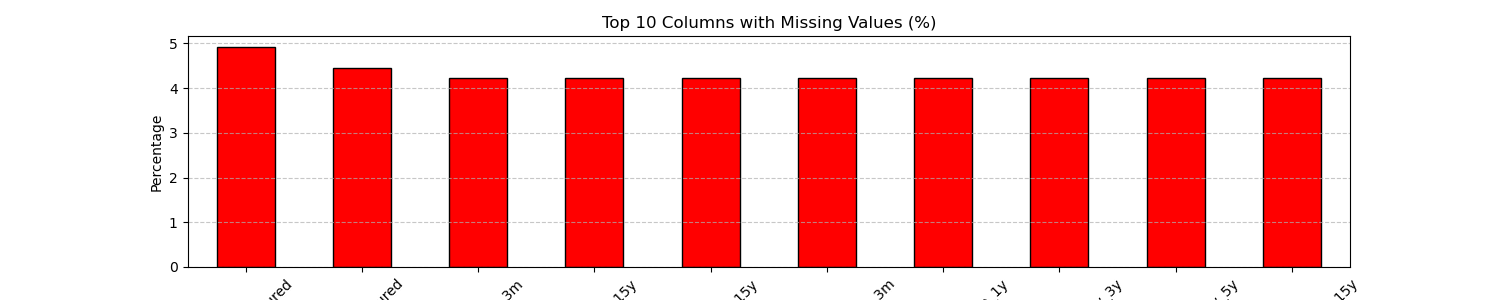
\includegraphics[width=1.0\textwidth]{\PathToOutput/wrds_premium_data.png}
    \caption{Overview of WRDS Premium Data. This dataset was manually extracted after initial WRDS datasets contained excessive missing values.}
\end{figure}

\subsection{Missing Data Analysis}
The missing data analysis highlights the extent of missing values across the initially pulled WRDS datasets. The figure below illustrates the percentage of missing data in each column, emphasizing the need for alternative data sources.

\begin{figure}[H]
    \centering
    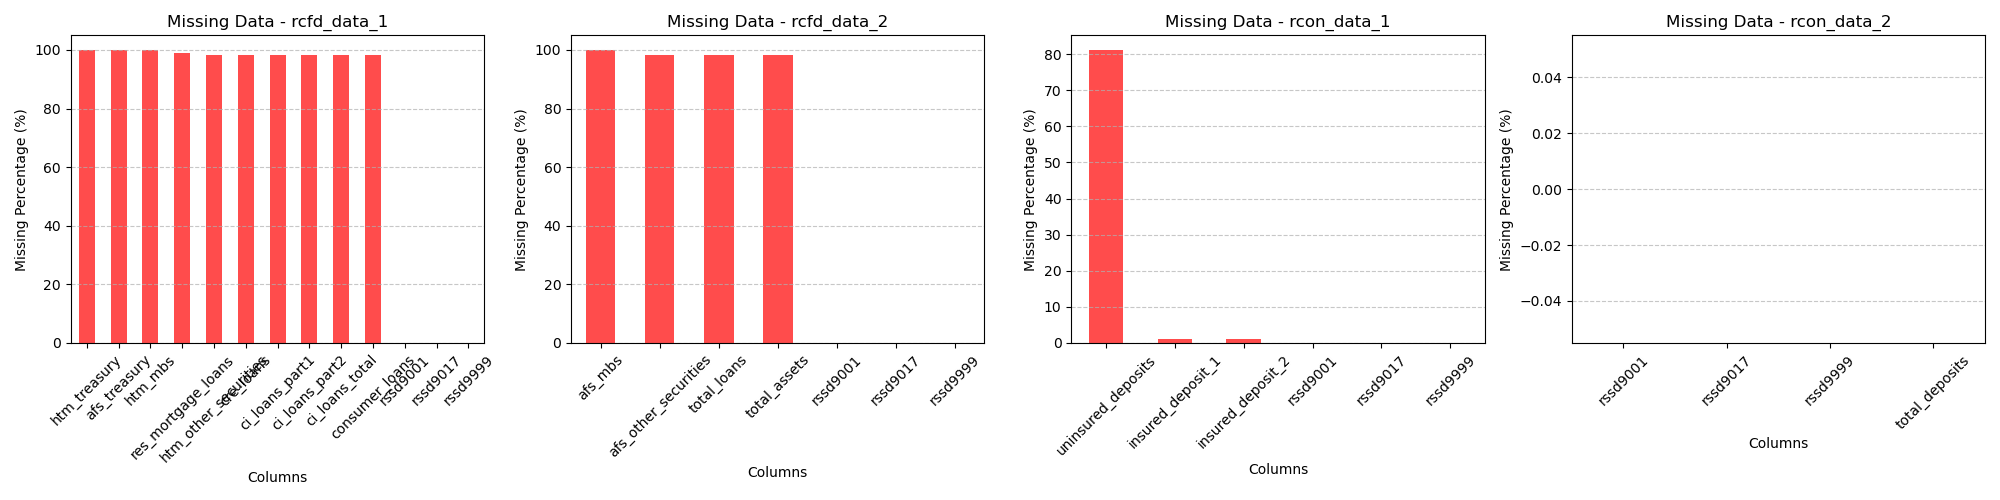
\includegraphics[width=1.0\textwidth]{\PathToOutput/missing_data.png}
    \caption{Percentage of Missing Data Across Different Datasets. The initial WRDS datasets showed over 90\% missing data in some tables, leading to the adoption of alternative data sources.}
\end{figure}

\section{Conclusion}
This report documents the steps taken to collect, clean, and analyze financial data. The integration of multiple sources ensures data reliability, while preprocessing and visualization facilitate meaningful insights. The decision to use the manually pulled WRDS bank premium data was crucial in ensuring a more complete and accurate dataset for further analysis.

\end{document}
